\chapter[Källtexter --- Kurvor]{Källtexter till Maple --- Kurvor}
\label{Reparametrize}

\emph{Reparametrize}-funktionen omparametriserar en plan algebraisk kurva givet på formen $C(t) = (f(t), g(t))$ till formen $(\pm t^n, g^*(t))$, där $n <= \mathbf{o}(g^*)$, eller till formen $(f^*(t), \pm t^n)$, där $n \leq \mathbf{o}(f^*)$. Funktionen använder två hjälpfunktioner; \emph{Composition} och \emph{MakePoly}, vilka beskrivs först. Sist i detta appendix följer några exempel på hur \emph{Reparametrize} kan användas i Maple.

\section{MakePoly}

\emph{MakePoly} tar en lista (array) av koefficienter och returnerar ett polynom i den valda variabeln. Ingående parametrar är:

\begin{table}[h]
\caption{Parametrar för \emph{MakePoly}}
\begin{center}
\begin{tabular}{|l|l|}
\hline
$a$ & En lista (array) med koefficienter.\\
$Variable$ & Namnet på variabeln som skall användas i polynomet.\\
\hline
\end{tabular}
\end{center}
\end{table}

\begin{verbatim}
MakePoly := proc(a, Variable)
   local i, r;

   r := 0;
   for i to nops(a) do 
      if op(i, a) <> 0 then
         r := r + op(i, a) * Variable^(i-1)
      fi
   od;

   RETURN(sort(r))
end\end{verbatim}

\subsection{Exempel}

\begin{maplegroup}
\begin{verbatim}
> MakePoly([1, 2, 3, 4, 5], x)
\end{verbatim}
\mapleresult
\begin{maplelatex}
\mapleinline{inert}{2d}{5*x^4+4*x^3+3*x^2+2*x+1}{\[\displaystyle 5\,{x}^{4}+4\,{x}^{3}+3\,{x}^{2}+2\,x+1\]}
\end{maplelatex}
\end{maplegroup}

\section{Composition}

\emph{Composition} beräknar kompositionen $f(g(t))$ av två polynom $f(t)$ och $g(t)$. Kompositionen beräknas bara upp till en viss grad för att spara på minne och tid.

Anledningen till att vi bara vill beräkna kompositionen $f(g(t))$ till en viss grad är att vi kanske redan vet att $f(t)$ och $g(t)$ bara har en viss grad av noggrannhet. I detta fall kommer kompositionen att ha samma grad av noggrannhet, och inte graden i kvadrat (vilken kan vara avsevärd).

För att göra det enklare att komma åt koefficienterna i den resulterande kompositionen, returneras resultatet som en array i stället för ett polynom. De ingående parametrarna är:

\begin{table}[h]
\caption{Parametrar för \emph{Composition}}
\begin{center}
\begin{tabular}{|l|l|}
\hline
$f$ & Polynomet $f(x)$ \\
$g$ & Polynomet $g(x)$ \\
$Variable$ & Namnet på variabeln som används. \\
$MaxDegree$ & Beräkning sker endast till denna grad. \\
\hline
\end{tabular}
\end{center}
\end{table}

\begin{verbatim}
Composition := proc(f, g, Variable, MaxDegree)
   local gc, gcn, gcnt, i, j, k, r, c, floop;

   gc := array(0..MaxDegree);
   gcn := array(0..MaxDegree);
   gcnt := array(0..MaxDegree);
   r := array(0..MaxDegree);

   for i from 0 to MaxDegree do
      gc[i] := coeff(g, Variable, i); 
      gcn[i] := gc[i]; 
      r[i] := 0
   od;

   floop := degree(f);
   if MaxDegree < floop then 
      floop := MaxDegree 
   fi;

   r[0] := coeff(f, Variable, 0);
   for i to floop do
      c := coeff(f, Variable, i);
      for j from 0 to MaxDegree do 
         r[j] := r[j] + c * gcn[j] 
      od;

      if i < MaxDegree then
         for j from 0 to MaxDegree do
            gcnt[j] := 0; 
            for k from 0 to j do
               gcnt[j] := gcnt[j] + gc[k] * gcn[j-k]
            od
         od;

         for j from 0 to MaxDegree do 
            gcn[j] := gcnt[j] 
         od
      fi
   od;

   RETURN(eval(r))
end
\end{verbatim}

\subsection{Exempel}

\begin{maplegroup}
\begin{verbatim}
> Composition(x^2+1, x^3+x^2+1, x, 6)
\end{verbatim}
\mapleresult
\begin{maplelatex}
\mapleinline{inert}{2d}{ARRAY([0 .. 6], [0 = 2, 1 = 0, 2 = 2, 3 = 2, 4 = 1, 5 = 2, 6 = 1])}{\[\displaystyle {\it ARRAY} \left( [{0\ldots 6}],[0=2,1=0,2=2,3=2,4=1,5=2,6=1] \right) \]}
\end{maplelatex}
\end{maplegroup}

\section{Reparametrize}

\emph{Reparametrize} tar en parametrisering av en kurva och skapar en ny parametrisering enligt algoritmen i sats \ref{ReparametrizeTheorem}. Parametrarna som krävs är följande:

\begin{table}[h]
\caption{Parametrar för \emph{Reparametrize}}
\begin{center}
\begin{tabular}{|l|p{9cm}|}
\hline
$x$ & Parametrisering av x-komponenten av kurvan. \\
$y$ & Parametrisering av y-komponenten av kurvan. \\
$Variable$ & Parametern (motsvarande $t$ i sats \ref{ReparametrizeTheorem}.\\
$t0$ & Runt vilken punkt kurvan skall parametriseras.\\
$MaxDegree$ & Till vilken grad omparametriseringen skall göras.\\
$Branch$ & Vilken gren som skall väljas som lösning. Standard är $0$.\\
$AllowNegation$ & Om omparametriseringen får innehålla $-t^n$ eller inte. Standard är \emph{true}.\\
\hline
\end{tabular}
\end{center}
\end{table}

\begin{verbatim}
Reparametrize := proc(x, y, Variable, t0 , MaxDegree, Branch,
   AllowNegation)
   local xt, yt, a, p, q, x0 , y0 , i, j, k, shifted, 
      temp, sols, StartTime, MinDegree, arg, z, Negate;

   StartTime := time();
   if not type(Branch, integer) then
      ERROR("Branch must be an integer!", Branch)
   fi;

   if t0 <> 0 then
      xt := collect(expand(convert(taylor(
         collect(expand(subs(Variable = Variable + t0, x)), 
         Variable), Variable = 0, MaxDegree + 1), polynom)), 
         Variable);

      yt := collect(expand(convert(taylor(
         collect(expand(subs(Variable = Variable + t0, y)), 
         Variable), Variable = 0, MaxDegree + 1), polynom)), 
         Variable)
   else
      xt := collect(expand(convert(taylor(x, Variable = 0, 
         MaxDegree + 1), polynom)), Variable);

      yt := collect(expand(convert(taylor(y, Variable = 0, 
         MaxDegree + 1), polynom)), Variable);
   fi;

   x0 := coeff(xt, Variable, 0);
   y0 := coeff(yt, Variable, 0);
   xt := xt - x0;
   yt := yt - y0;
   MinDegree := ldegree(xt, Variable);
   shifted := ldegree(yt, Variable) < MinDegree;

   if shifted then
      temp := xt; 
      xt := yt; 
      yt := temp; 
      MinDegree := ldegree(xt, Variable)
   fi;

   a := array(1..MaxDegree - MinDegree + 1);
   z := 1/coeff(xt, Variable, MinDegree);
   if z < 0 and AllowNegation then 
      xt := -xt; 
      z := -z; 
      Negate := true
   else 
      Negate := false
   fi;

   arg := argument(z);
   a[1] := abs(z)^(1/MinDegree) * (
      cos((2 * (MinDegree - 2 + Branch) * Pi + arg)/MinDegree)
      + I * sin((2 * (MinDegree - 2 + Branch) * Pi + arg)/MinDegree));

   p := a[1] * Variable;
   for j from 2 to MaxDegree - MinDegree + 1 do 
      p := p + a[j] * Variable^j 
   od;

   q := Composition(yt, p, Variable, MaxDegree);
   p := Composition(xt, p, Variable, MaxDegree);
   i := MinDegree + 1;
   j := 2;

   while i <= MaxDegree do
      sols := [solve(p[i] = 0, a[j])];
      q[i] := expand(subs(a[j] = sols[1], q[i]));

      if i < MaxDegree then
         for k from i + 1 to MaxDegree do
            p[k] := subs(a[j] = sols[1], p[k]); 
            q[k] := subs(a[j] = sols[1], q[k])
         od
      fi;

      a[j] := sols[1];
      i := i + 1;
      j := j + 1
   od;

   xt := q[0];
   for i to MaxDegree do 
      if q[i] <> 0 then 
         xt := xt + q[i] * Variable^i 
      fi 
   od;

   if shifted then
      xt := x0 + xt;
      if Negate then 
         yt := y0 - Variable^MinDegree
      else 
         yt := y0 + Variable^MinDegree
      fi
   else
      yt := y0 + xt;
      if Negate then 
         xt := x0 - Variable^MinDegree
      else 
         xt := x0 + Variable^MinDegree
      fi
   fi;

   printf("Elapsed Time: %0.3f s.\n", time() - StartTime);

   RETURN([xt, yt])
end
\end{verbatim}

\subsection{Exempel --- Ett första}
\label{ReparametrizeEx1}
Kurvan $(t^2+t^3,t^5+t^6)$ har en singularitet i $t = 0$. Dessutom passerar kurvan genom origo då $t = -1$. Först ber vi Maple att parametrisera om kurvan kring $t = 0$:

\begin{maplegroup}
\begin{verbatim}
> Reparametrize(t^3+t^2, t^6+t^5, t, 0, 10, 0, false);

Elapsed Time: 0.016 s.
\end{verbatim}
\mapleresult
\begin{maplelatex}
\mapleinline{inert}{2d}{[t^2, t^5-(3/2)*t^6+(21/8)*t^7-5*t^8+(1287/128)*t^9-21*t^10]}{\[\displaystyle [{t}^{2},{t}^{5}-3/2\,{t}^{6}+{\frac {21\,{t}^{7}}{8}}-5\,{t}^{8}+{\frac {1287\,{t}^{9}}{128}}-21\,{t}^{10}]\]}
\end{maplelatex}
\end{maplegroup}

\vspace{20pt}
Därefter vill vi ha en omparametrisering kring $t = -1$:

\begin{maplegroup}
\begin{verbatim}
> Reparametrize(t^3+t^2, t^6+t^5, t, -1, 10, 0, false);

Elapsed Time: 0.016 s.
\end{verbatim}
\mapleresult
\begin{maplelatex}
\mapleinline{inert}{2d}{[t, 163438*t^10+29070*t^9+5304*t^8+1001*t^7+198*t^6+42*t^5+10*t^4+3*t^3+3*t^2-t]}{\[\displaystyle [t,163438\,{t}^{10}+29070\,{t}^{9}+5304\,{t}^{8}+1001\,{t}^{7}+198\,{t}^{6}+42\,{t}^{5}+10\,{t}^{4}+3\,{t}^{3}+3\,{t}^{2}\\
\mbox{}-t]\]}
\end{maplelatex}
\end{maplegroup}

\vspace{20pt}
Ritar vi ut originalparametriseringen av kurvan (prickad tjock linje) och de två omparametriseringarna (tunna hela linjer) i samma graf får vi:

\begin{center}
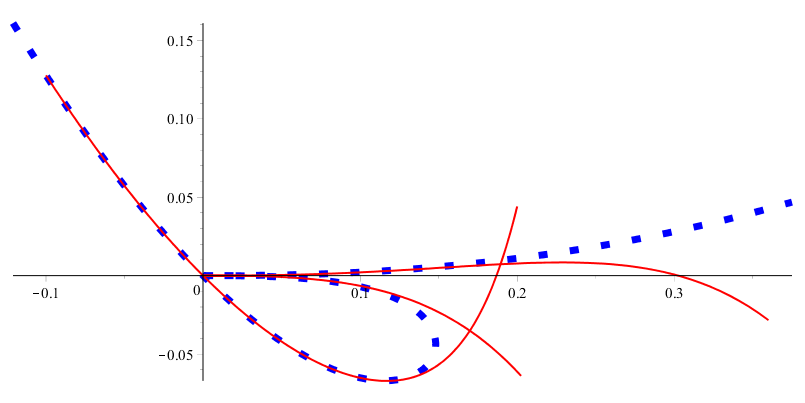
\includegraphics[scale=0.35]{Export/kurvorplot2d1.png}
\end{center}

\subsection{Exempel --- Byte av axel}

Ellipsen $\left(3 \sin(t), 2 \cos(t)\right)$ saknar singulariteter, men vi kan parametrisera om kurvan ändå. Notera hur omparametriseringarna skiljer från $t=0$ och $t=\pi$, jämfört med $t=\pm \pi/2$:

\begin{maplegroup}
\begin{verbatim}
> Reparametrize(3*sin(t), 2*cos(t), t, 0, 10, 0, false);

Elapsed Time: 0.015 s.
\end{verbatim}
\mapleresult
\begin{maplelatex}
\mapleinline{inert}{2d}{[t, 2-(1/9)*t^2-(1/324)*t^4-(1/5832)*t^6-(5/419904)*t^8-(7/7558272)*t^10]}{\[\displaystyle \left[t,2-1/9\,{t}^{2}-{\frac {{t}^{4}}{324}}-{\frac {{t}^{6}}{5832}}-{\frac {5\,{t}^{8}}{419904}}-{\frac {7\,{t}^{10}}{7558272}}\right]\]}
\end{maplelatex}
\end{maplegroup}

\begin{maplegroup}
\begin{verbatim}
> Reparametrize(3*sin(t), 2*cos(t), t, Pi, 10, 0, false);

Elapsed Time: 0.016 s.
\end{verbatim}
\mapleresult
\begin{maplelatex}
\mapleinline{inert}{2d}{[t, -2+(1/9)*t^2+(1/324)*t^4+(1/5832)*t^6+(5/419904)*t^8+(7/7558272)*t^10]}{\[\displaystyle \left[t,-2+1/9\,{t}^{2}+{\frac {{t}^{4}}{324}}+{\frac {{t}^{6}}{5832}}+{\frac {5\,{t}^{8}}{419904}}+{\frac {7\,{t}^{10}}{7558272}}\right]\]}
\end{maplelatex}
\end{maplegroup}

\begin{maplegroup}
\begin{verbatim}
> Reparametrize(3*sin(t), 2*cos(t), t, (1/2)*Pi, 10, 0, false);

Elapsed Time: 0.016 s.
\end{verbatim}
\mapleresult
\begin{maplelatex}
\mapleinline{inert}{2d}{[3-(3/8)*t^2-(3/128)*t^4-(3/1024)*t^6-(15/32768)*t^8-(21/262144)*t^10, t]}{\[\displaystyle \left[3-3/8\,{t}^{2}-{\frac {3\,{t}^{4}}{128}}-{\frac {3\,{t}^{6}}{1024}}-{\frac {15\,{t}^{8}}{32768}}-{\frac {21\,{t}^{10}}{262144}},t\right]\]}
\end{maplelatex}
\end{maplegroup}

\begin{maplegroup}
\begin{verbatim}
> Reparametrize(3*sin(t), 2*cos(t), t, -(1/2)*Pi, 10, 0, false);

Elapsed Time: 0.015 s.
\end{verbatim}
\mapleresult
\begin{maplelatex}
\mapleinline{inert}{2d}{[-3+(3/8)*t^2+(3/128)*t^4+(3/1024)*t^6+(15/32768)*t^8+(21/262144)*t^10, t]}{\[\displaystyle \left[-3+3/8\,{t}^{2}+{\frac {3\,{t}^{4}}{128}}+{\frac {3\,{t}^{6}}{1024}}+{\frac {15\,{t}^{8}}{32768}}+{\frac {21\,{t}^{10}}{262144}},t\right]\]}
\end{maplelatex}
\end{maplegroup}

\vspace{20pt}
Ritar vi sedan ut originalparametriseringen av kurvan tillsammans med de fyra omparametriseringarna får vi:

\begin{center}
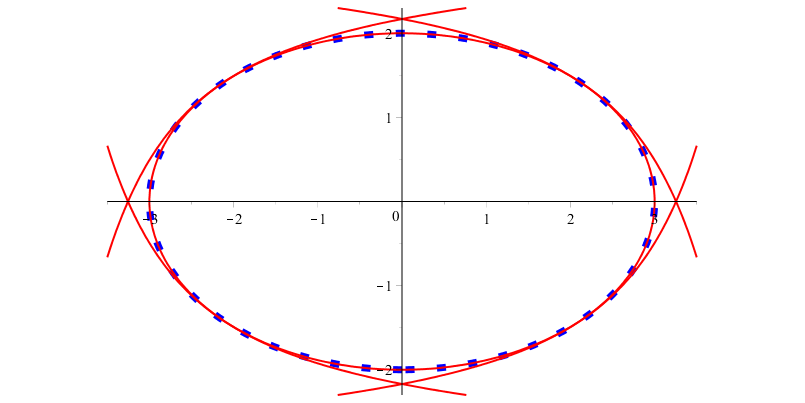
\includegraphics[scale=0.35]{Export/kurvorplot2d2.png}
\end{center}

\subsection{Exempel --- Singulariteter}
\label{ReparametrizeSingularities}

Kurvan $\left(t^3(t - 1)^3(t + 1)^3,t^5(t - 1)^2(t + 1)^2\right) = \left(t^9 - 3t^7 + 3t^5 - t^3, t^5 - 2t^7 + t^9\right)$ har en singularitet i $t = 0$ av ordning $2$, en i $t = 1$ av ordning $1$
och en i $t = -1$ av ordning $1$. Vi analyserar hur omparametriseringarna uppför sig i dessa tre singulariteter:

\begin{maplegroup}
\begin{verbatim}
> Reparametrize(t^3*(t-1)^3*(t+1)^3, t^5*(t-1)^2*(t+1)^2, t, 0, 15,
0, false);

Elapsed Time: 0.031 s.
\end{verbatim}
\mapleresult
\begin{maplelatex}
\mapleinline{inert}{2d}{[t^3, -1428*t^15-273*t^13-55*t^11-12*t^9-3*t^7-t^5]}{\[\displaystyle \left[{t}^{3},-1428\,{t}^{15}-273\,{t}^{13}-55\,{t}^{11}-12\,{t}^{9}-3\,{t}^{7}-{t}^{5}\right]\]}
\end{maplelatex}
\end{maplegroup}

\begin{maplegroup}
\begin{verbatim}
> Reparametrize(t^3*(t-1)^3*(t+1)^3, t^5*(t-1)^2*(t+1)^2, t, 1, 15, 
0, false);

Elapsed Time: 0.063 s.
\end{verbatim}
\mapleresult
\begin{maplelatex}
\mapleinline{inert}{2d}{[(1/2)*sqrt(4)*t^3-(9/4)*t^4+(207/64)*sqrt(4)*t^5-21*t^6+(150183/4096)*sqrt(4)*t^7-(137655/512)*t^8+(66893079/131072)*sqrt(4)*t^9-3978*t^10+(132735945771/16777216)*sqrt(4)*t^11-(8385901667/131072)*t^12+(70379121262905/536870912)*sqrt(4)*t^13-(4345965/4)*t^14+(78087826643607459/34359738368)*sqrt(4)*t^15, t^2]}{\[\displaystyle
\begin{array}{l}
\left[1/2\, \sqrt{4}{t}^{3}-9/4\,{t}^{4}+{\frac {207\, \sqrt{4}{t}^{5}}{64}}-21\,{t}^{6}+{\frac {150183\, \sqrt{4}{t}^{7}}{4096}}\right. \\
\mbox{}-{\frac {137655\,{t}^{8}}{512}}+{\frac {66893079\, \sqrt{4}{t}^{9}}{131072}}-3978\,{t}^{10}+{\frac {132735945771\, \sqrt{4}{t}^{11}}{16777216}}\\
\mbox{}-{\frac {8385901667\,{t}^{12}}{131072}}+{\frac {70379121262905\, \sqrt{4}{t}^{13}}{536870912}}\\
\left.\mbox{}-{\frac {4345965\,{t}^{14}}{4}}+{\frac {78087826643607459\, \sqrt{4}{t}^{15}}{34359738368}},{t}^{2}\right]
\end{array}\]}
\end{maplelatex}
\end{maplegroup}

\begin{maplegroup}
\begin{verbatim}
> Reparametrize(t^3*(t-1)^3*(t+1)^3, t^5*(t-1)^2*(t+1)^2, t, -1, 15, 
0, true);

Elapsed Time: 0.047 s.
\end{verbatim}
\mapleresult
\begin{maplelatex}
\mapleinline{inert}{2d}{[(1/2)*sqrt(4)*t^3+(9/4)*t^4+(207/64)*sqrt(4)*t^5+21*t^6+(150183/4096)*sqrt(4)*t^7+(137655/512)*t^8+(66893079/131072)*sqrt(4)*t^9+3978*t^10+(132735945771/16777216)*sqrt(4)*t^11+(8385901667/131072)*t^12+(70379121262905/536870912)*sqrt(4)*t^13+(4345965/4)*t^14+(78087826643607459/34359738368)*sqrt(4)*t^15, -t^2]}{\[\displaystyle
\begin{array}{l}
\left[1/2\, \sqrt{4}{t}^{3}+9/4\,{t}^{4}+{\frac {207\, \sqrt{4}{t}^{5}}{64}}+21\,{t}^{6}+{\frac {150183\, \sqrt{4}{t}^{7}}{4096}}\right.\\
\mbox{}+{\frac {137655\,{t}^{8}}{512}}+{\frac {66893079\, \sqrt{4}{t}^{9}}{131072}}+3978\,{t}^{10}+{\frac {132735945771\, \sqrt{4}{t}^{11}}{16777216}}\\
\mbox{}+{\frac {8385901667\,{t}^{12}}{131072}}+{\frac {70379121262905\, \sqrt{4}{t}^{13}}{536870912}}\\
\left.\mbox{}+{\frac {4345965\,{t}^{14}}{4}}+{\frac {78087826643607459\, \sqrt{4}{t}^{15}}{34359738368}},-{t}^{2}\right]
\end{array}\]}
\end{maplelatex}
\end{maplegroup}

\vspace{20pt}
Ritar vi sedan ut originalparametriseringen av kurvan tillsammans med de tre omparametriseringarna får vi följande intressanta bild:

\begin{center}
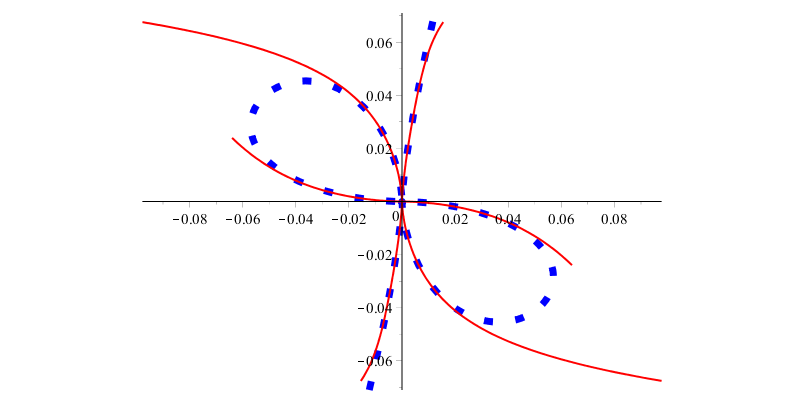
\includegraphics[scale=0.35]{Export/kurvorplot2d3.png}
\end{center}

\subsection{Exempel --- Negering}

Kurvan $\left(t^3 - t^2,t^3 + t^2\right)$ har en singularitet av ordning $1$ i $t = 0$. Vi använder Maple för att omparametrisera kurvan i denna punkt:

\begin{maplegroup}
\begin{verbatim}
> Reparametrize(t^3-t^2, t^3+t^2, t, 0, 10, 0, true);

Elapsed Time: 0.000 s.
\end{verbatim}
\mapleresult
\begin{maplelatex}
\mapleinline{inert}{2d}{[-t^2, 3*t^4+2*t^3+t^2+(21/4)*t^5+10*t^6+(1287/64)*t^7+42*t^8+(46189/512)*t^9+198*t^10]}{\[\displaystyle \left[-{t}^{2},3\,{t}^{4}+2\,{t}^{3}+{t}^{2}+{\frac {21\,{t}^{5}}{4}}+10\,{t}^{6}+{\frac {1287\,{t}^{7}}{64}}+42\,{t}^{8}+{\frac {46189\,{t}^{9}}{512}}+198\,{t}^{10}\right]\]}
\end{maplelatex}
\end{maplegroup}

\vspace{20pt}
Som man kan se av omparametriseringen blir x-termen $-t^2$. Man kan be Maple att omparametrisera kurvan så att x-termen blir positiv. Detta
medför givetvis att y-termen får komplexa koefficienter:

\begin{maplegroup}
\begin{verbatim}
> Reparametrize(t^3-t^2, t^3+t^2, t, 0, 10, 0, false);

Elapsed Time: 0.031 s.
\end{verbatim}
\mapleresult
\begin{maplelatex}
\mapleinline{inert}{2d}{[t^2, -t^2-(2*I)*t^3+3*t^4+(21/4*I)*t^5-10*t^6-(1287/64*I)*t^7+42*t^8+(46189/512*I)*t^9-198*t^10]}{\[\displaystyle
\begin{array}{l}
\left[{t}^{2},-{t}^{2}-2\,i{t}^{3}+3\,{t}^{4}+{\frac {21\,i}{4}}{t}^{5}\right.\\
\left.\mbox{}-10\,{t}^{6}-{\frac {1287\,i}{64}}{t}^{7}+42\,{t}^{8}+{\frac {46189\,i}{512}}{t}^{9}-198\,{t}^{10}\right]
\end{array}\]}
\end{maplelatex}
\end{maplegroup}

\vspace{20pt}
Om vi plottar den ursprungliga funktionen och dess reellvärda omparametrisering tillsammans med realdelen och imaginärdelen av den komplexa omparametriseringen var för sig (tunna punkt-streckade linjer), får vi följande graf:

\begin{center}
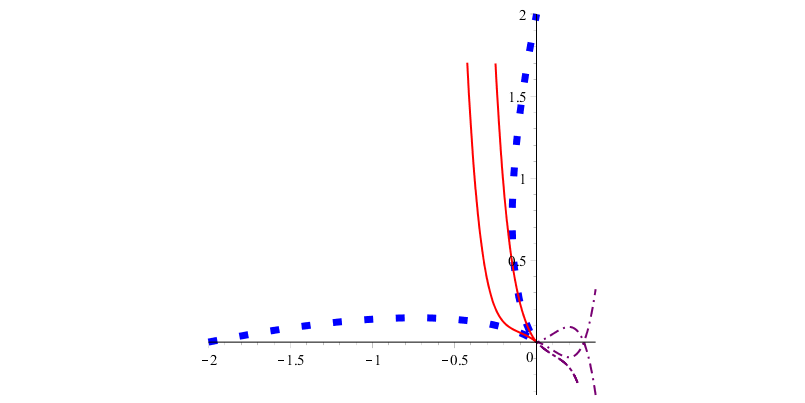
\includegraphics[scale=0.35]{Export/kurvorplot2d4.png}
\end{center}

\subsection{Exempel --- Udda ordning}

Kurvan $\left(t^4 - t^3,t^4 + t^3\right)$ har en singularitet av ordning $2$ i $t = 0$. Den liknar mycket kurvan i exemplet ovan, men eftersom ordningen av x- och y-termerna är udda ($3$), kommer omparametriseringen att vara reell utan att x-termen måste negeras. Vi använder Maple för att omparametrisera kurvan:

\begin{maplegroup}
\begin{verbatim}
> Reparametrize(t^4-t^3, t^4+t^3, t, 0, 10, 2, true);

Elapsed Time: 0.016 s.
\end{verbatim}
\mapleresult
\begin{maplelatex}
\mapleinline{inert}{2d}{[-t^3, 2*t^4+t^3+(8/3)*t^5+4*t^6+(520/81)*t^7+(2618/243)*t^8+(56/3)*t^9+(217360/6561)*t^10]}{\[\displaystyle \left[-{t}^{3},2\,{t}^{4}+{t}^{3}+8/3\,{t}^{5}+4\,{t}^{6}+{\frac {520\,{t}^{7}}{81}}+{\frac {2618\,{t}^{8}}{243}}+{\frac {56\,{t}^{9}}{3}}+{\frac {217360\,{t}^{10}}{6561}}\right]\]}
\end{maplelatex}
\end{maplegroup}

\vspace{20pt}
Vi kan också parametrisera om kurvan utan en negativ $t^n$ komponent. Eftersom ordningen hos komponenterna är udda, kommer bara de udda termerna byta tecken, och komplexa termer undvikas: 

\begin{maplegroup}
\begin{verbatim}
> Reparametrize(t^4-t^3, t^4+t^3, t, 0, 10, 0, false);

Elapsed Time: 0.015 s.
\end{verbatim}
\mapleresult
\begin{maplelatex}
\mapleinline{inert}{2d}{[t^3, 2*t^4-t^3-(8/3)*t^5+4*t^6-(520/81)*t^7+(2618/243)*t^8-(56/3)*t^9+(217360/6561)*t^10]}{\[\displaystyle \left[{t}^{3},2\,{t}^{4}-{t}^{3}-8/3\,{t}^{5}+4\,{t}^{6}-{\frac {520\,{t}^{7}}{81}}+{\frac {2618\,{t}^{8}}{243}}-{\frac {56\,{t}^{9}}{3}}+{\frac {217360\,{t}^{10}}{6561}}\right]\]}
\end{maplelatex}
\end{maplegroup}

\vspace{20pt}
Om vi plottar den ursprungliga kurvan och dess två parametriseringar (dessa två ger samma kurva), får vi följande graf:

\begin{center}
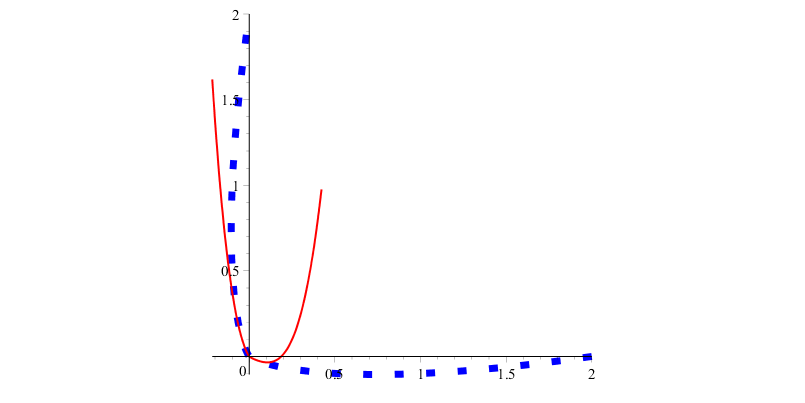
\includegraphics[scale=0.35]{Export/kurvorplot2d5.png}
\end{center}
